\chapter{Revisão Bibliográfica}

No presente capítulo, são apresentados conceitos básico para a compreensão do presente trabalho. Nessa etapa, busca-se através da revisão de trabalhos já elucidados a contextualização do projeto proposto.

%%%%%%%%%%%%%%%%%%%%%%%%%%%%%%%%%%%%%%%%%%%%%%%%%%%%%%%%%%%%%%%%%%%%%%
\section{Satélites Artificiais} %ch 1303


%%%%%%%%%%%%%%%%%%%%%%%%%%%%%%%%%%%
\subsection{Dinâmica de um Satélite}

%%%%%%%%%%%%%%%%%%%%%%%%%%%%%%%%%%%
\subsubsection{Dinâmica de Corpo Rígido}

%%%%%%%%%%%%%%%%%%%%%%%%%%%%%%%%%%%
\subsubsection{Dinâmica de Translação}

%%%%%%%%%%%%%%%%%%%%%%%%%%%%%%%%%%%
\subsubsection{Dinâmica de Rotação}

\subsubsection{Matriz de Rotação}

\subsection{Controle Tridimensional do Satélite}

\subsubsection{Rodas de Reação}

\begin{figure}[!ht]
  \caption{Representação Mecânica Simplificada de um satélite com rodas de Reação.}
  \begin{center}
      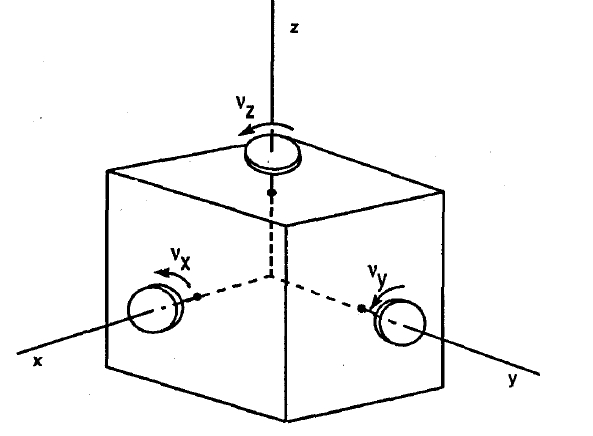
\includegraphics[scale=0.75]{img/satellite_controlhand_p1306}
  \end{center}
  \fonte{Adaptado de \citeonline{Levine1996}.} 
  \label{fig:satellite_controlhand_p1306}
\end{figure}



%%%%%%%%%%%%%%%%%%%%%%%%%%%%%%%%%%%%%%%%%%%%%%%%%%%%%%%%%%%%%%%%%%%%%%
%conceitos de resposta em frequência
% estabilidade de sistemas
% em regime
% diferentes tipos de sistemas

%%%%%%%%%%%%%%%%%%%%%%%%%%%%%%%%%%%%%%%%%%%%%%%%%%%%%%%%%%%%%%%%%%%%%%
\section{Controlador PID}

\subsection{Resposta ao Degrau do um Sistema}

Um problema fundamental em engenharia, é prever e modelar sistemas naturais ou artificias para tirarmos o melhor proveito de suas características. Para isso, muitas técnicas foram desenvolvidas para se conseguir controlar essas variáveis de interesse \cite{Levine1996}.

Uma forma clássica de representar um resposta de uma variável de interesse, é através da resposta ao degrau. Essa pode ser vista na figura \ref{fig:transient_ogata_p170}, onde temos as principais características da resposta ao degrau de um sistema de segunda ordem ou superior. Onde \textit{$M_p$} (maximum overshoot) é o sobressinal do da variável de interesse em percentual, \textit{$t_d$} (delay Time) é o tempo atraso de transporte, \textit{$t_r$} (rise time) é o tempo necessário para atingir o valor do sinal de referência, \textit{$t_p$} é o tempo de pico (peak time) e \textit{$t_s$} (settling time) é o tempo para o sistema entrar em regime, observando um critério de erro em regime \cite{Ogata}.

\begin{figure}[!ht]
  \caption{Parâmetros de uma Resposta ao Degrau de um sistema de segunda ordem ou superior.}
  \begin{center}
      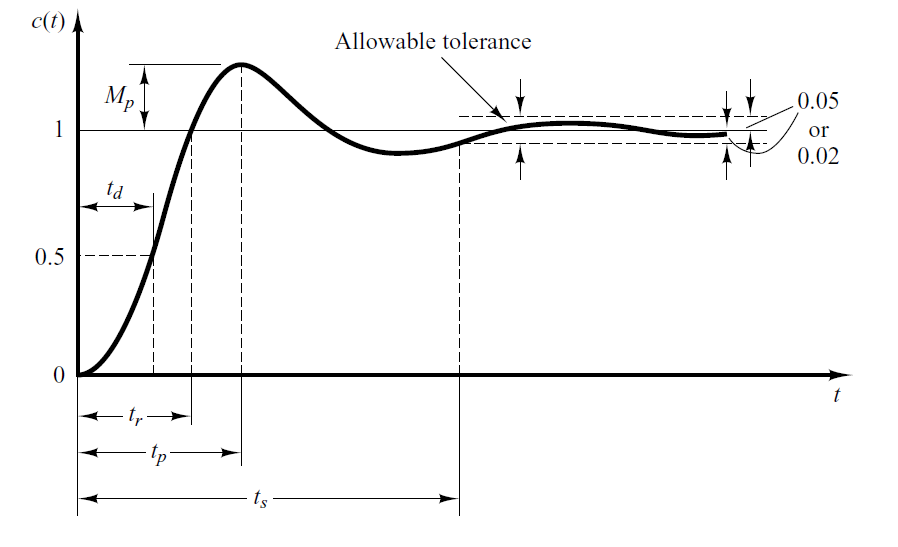
\includegraphics[scale=0.5]{img/transient_ogata_p170}
  \end{center}
  \fonte{Adaptado de \citeonline{Ogata}.} 
  \label{fig:transient_ogata_p170}
\end{figure}

A resposta ao degrau nos diz muito sobre os sistemas de interesse, pois nela podemos ver claramente a atuação dos \textit{polos} e \textit{zeros} dominantes e o ganho de baixa frequência da função de transferência do sistema. Os métodos clássicos para se calcular os parâmetros de controladores são baseados na resposta ao degrau \cite{Ogata}. 

%%%%%%%%%%%%%%%%%%%%%%%%%%%%%%%%%%%
\subsection{Controlador PID}

O controlador proporcional-integral-derivativo é um dos controladores mais utilizados nas aplicações industriais. Essa topologia de controlador consegue, em diferentes configurações atender entre 90 e 95\% de todos os sistemas que necessitam de controladores \cite{Levine1996}. A forma descritiva matemática mais comum de se encontrar um controlador PID no domínio do tempo é a seguinte:

\begin{gather}
  u(t) = K\left((e(t)+\frac{1}{T_i}\int_{0}^{t}{e(\tau)}d\tau+T_d\frac{de(t)}{dt}\right) 
\end{gather}

Onde \textit{e(t)} é o erro, \textit{$T_i$} é o tempo integral, \textit{$T_d$} é o tempo derivativo e \textit{K} o ganho proporcional. Uma outra forma de se representar os tempos integral e derivativo, é através dos ganhos \textit{$K_i$} que é o ganho integral e o \textit{$K_d$}, que é o ganho derivativo \cite{Astrom1995};


Na figura \ref{fig:pid_controller_Snider_p35}, podemos ver a configuração mais utilizada do controlador PID, onde $\beta_{com}(S)$ é o valor do sinal de referência no domínio da frequência, \textit{err(S)} o erro, \textit{$K_p$} é o ganho proporcional, \textit{$K_i$} é o ganho integral, \textit{$K_d$} é o ganho derivativo, \textit{$G_e(s)$} é a função de transferência do controlador PID, \textit{$M_{c1}(s)$} é o sinal de erro tratado pelo controlador, \textit{D(S)} é um distúrbio, \textit{$G_p(S)$} é a função de transferência da planta e por fim, \textit{$\beta(S)$} que é a variável de interesse \cite{Snider}.

\begin{figure}[!ht]
  \caption{Representação do Modelo de Controlador PID com distúrbios.}
  \begin{center}
      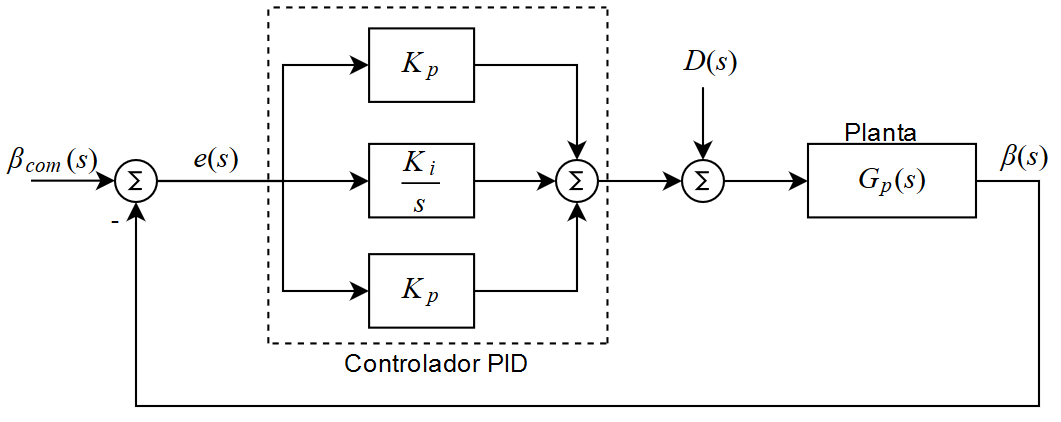
\includegraphics[scale=0.75]{img/pid_controller_Snider_p35}
  \end{center}
  \fonte{\citeonline{Snider}.} 
  \label{fig:pid_controller_Snider_p35}
\end{figure}

Como alguns sistemas podem admitir grandes e rápidas variações de sinais de referência, exigindo uma grande força de controle e energia no atuador, algumas topologias foram desenvolvidas para limitar a atuação de alguns fatores dos controladores. Um bom exemplo é o \textit{anti-windup}, onde essa topologia limita a saturação do atuador quando o sistema atinge o regime, causado pela ação integral. Essa topologia pode ser vista no modelo da figura \ref{fig:pid_antiwindup_astrom_p83} \cite{Astrom1995}.

\begin{figure}[!ht]
  \caption{Modelo de um Controlador PID com Histerese}
  \begin{center}
      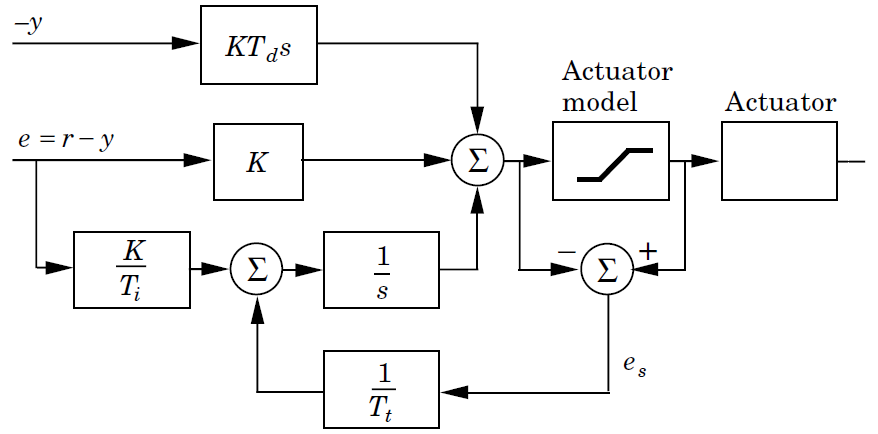
\includegraphics[scale=0.65]{img/pid_antiwindup_astrom_p83}
  \end{center}
  \fonte{\citeonline{Astrom1995}.} 
  \label{fig:pid_antiwindup_astrom_p83}
\end{figure}

Existem muitas combinações de controladores PID, cada uma com suas peculiaridades e vantagens de uso. Uma combinação muito usada é a PI, onde a acão integral de zerar o erro em regime e uma boa resposta transitória já satisfazem as especificações. Podemos ver um exemplo dessa configuração na imagem \ref{fig:pi_twomotors_astrom_p308}, onde apenas um controlador PI controla a velocidade angular (\textit{$\omega$})somada de dois motores (Motor 1 e Motor 2) a partir de uma velocidade de referência (\textit{$\omega_{sp}$}) \cite{Astrom1995}.

\begin{figure}[!ht]
  \caption{Representação do Modelo de Controlador PI com dois motores.}
  \begin{center}
      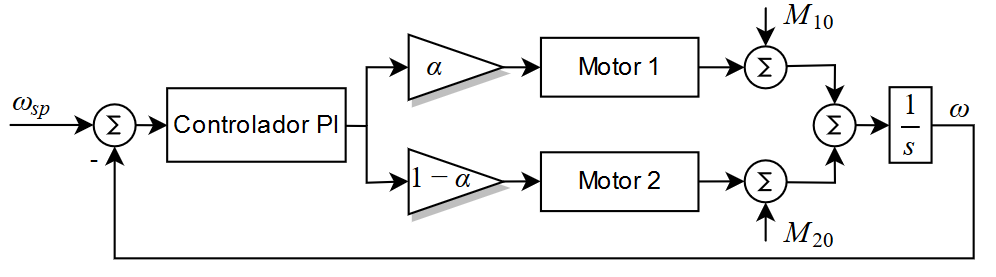
\includegraphics[scale=0.65]{img/pi_twomotors_astrom_p308}
  \end{center}
  \fonte{Adaptado de \citeonline{Astrom1995}.} 
  \label{fig:pi_twomotors_astrom_p308}
\end{figure}

%%%%%%%%%%%%%%%%%%%%%%%%%%%%%%%%%%%%%%%%%%%%%%%%%%%%%%%%%%%%%%%%%%%%%%
\section{Sintonia de Controladores}

Como podemos ver no modelo matemático e gráfico dos controladores PID, os valores de ajuste $K_p$, $T_i$ e $T_d$  podem assumir infinitos valores, sendo necessário a escolha do melhor conjunto desses valores para que a planta desempenhe o comportamento esperado \cite{Ogata}.


%%%%%%%%%%%%%%%%%%%%%%%%%%%%%%%%%%%
\subsection{Método de sintonia de Ziegler-Nichols}

Dois métodos clássicos de sintonia foram desenvolvidos em 1942 por Ziegler e Nichols. Esses dois métodos são baseados em características da resposta ao degrau e o com a resposta em frequência. Na figura \ref{fig:ziegler-nichols_astrom_p135} podemos ver a resposta ao degrau e os parâmetros de atraso (L) e velocidade da resposta (a), que são usados para o cálculos dos parâmetros do controlador  \cite{Astrom1995}. 

\begin{figure}[!ht]
  \caption{Resposta ao degrau e os parâmetros de atraso (L) e velocidade da resposta (a).}
  \begin{center}
      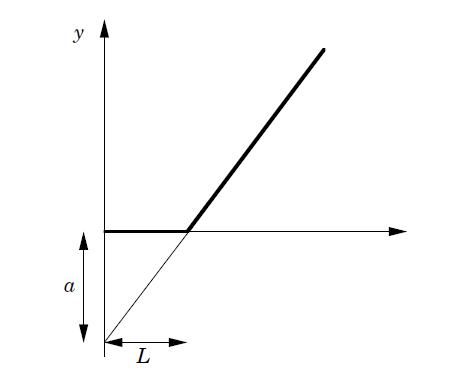
\includegraphics[scale=0.75]{img/ziegler-nichols_astrom_p135}
  \end{center}
  \fonte{\citeonline{Astrom1995}.} 
  \label{fig:ziegler-nichols_astrom_p135}
\end{figure}

Na tabela \ref{tab:Ziegler-Nichols} podemos ver as relações dos parâmetros $K_p$, $T_i$, $T_d$ e $T_p$ com os vistos na figura \ref{fig:ziegler-nichols_astrom_p135}.  

\begin{table}
  \caption{Parâmetros PID pelo Método de Ziegler-Nichols - Resposta ao Degrau}
  \label{tab:Ziegler-Nichols}
  \centering%
  \begin{minipage}{.42\textwidth}
    \begin{tabular*}{\textwidth}{lllll}
      \hline
      {Controlador} & {K} & {$T_i$} & {$T_d$}& {$T_p$}\\ \hline
      \hline
      P    &  1/a   &     &      & 4L  \\ 
      PI   &  0.9/a & 3L  &      & 5.7L  \\
      PID  &  1.2/a & 2L  & L/2  & 3.4L  \\ \hline
    \end{tabular*}
    \fonte{Adaptado de \citeonline{Astrom1995}}
  \end{minipage}
\end{table}

O outro método de se estimar os valores do controlador, é através de duas características da resposta em frequência: uma delas que é o ganho que deixa o sistema marginalmente estável ($K_u$), e a outra, é o período do sinal de referência que deixa o sistema marginalmente estável ($T_u$). Podemos ver na tabela \ref{tab:Ziegler-Nichols-freq} as relações entre $K_p$, $T_i$, $T_d$, $T_p$ e ($K_u$) e ($T_u$) . 

\begin{table}
  \caption{Parâmetros PID pelo Método de Ziegler-Nichols - Resposta em Frequência}
  \label{tab:Ziegler-Nichols-freq}
  \centering%
  \begin{minipage}{.6\textwidth}
    \begin{tabular*}{\textwidth}{lllll}
      \hline
      {Controlador} & {K} & {$T_i$} & {$T_d$}& {$T_p$}\\ \hline
      \hline
      P    &  0.5$K_u$   &           &             & $T_u$  \\ 
      PI   &  0.4$K_u$   & 0.8$T_u$  &             & 1.4$T_u$ \\
      PID  &  0.6$K_u$   & 0.5$T_u$  & 0.125$T_u$  & 0.85$T_u$  \\ \hline
    \end{tabular*}
    \fonte{Adaptado de \citeonline{Astrom1995}}
  \end{minipage}
\end{table}

%\subsection{Métodos de Otimização ????}
%%%%%%%%%%%%%%%%%%%%%%%%%%%%%%%%%%%%%%%%%%%%%%%%%%%%%%%%%%%%%%%%%%%%%%
\subsection{Sintonia Automática de Controladores e Controle Adaptativo}


Como muitos sistemas sofrem variações temporais, distúrbios e o interesse do usuário em modificar constantemente a resposta da planta, cria-se a necessidade de automatizar o processo de sintonia, ao um simples comando do usuário.

Além da simplicidade do conceito de implementação, os controladores PID são muito utilizados pela possibilidade de auto sintonia e adaptatividade dos controladores, pois a partir do comportamento da resposta ao degrau podemos calcular os parâmetros do controlador e aplicarmos sem a intervenção humana\cite{Astrom1995}. Na figura \ref{fig:pid_adaptative_astrom_p233}, podemos a partir do comportamento da planta, escolher a ou as técnicas mais adequadas que devemos implementar para controlar de forma satisfatória a planta.

\begin{figure}[!ht]
  \caption{Fluxograma para a escolha do Método de Sintonia.}
  \begin{center}
      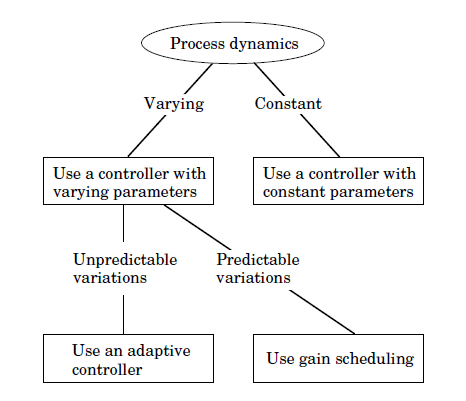
\includegraphics[scale=0.75]{img/escolha_controle_astrom_p236}
  \end{center}
  \fonte{Adaptado de \citeonline{Astrom1995}.} 
  \label{fig:pid_adaptative_astrom_p233}
\end{figure}


%%%%%%%%%%%%%%%%%%%%%%%%%%%%%%%%%%%
\subsubsection{Método do Relé}

Características da resposta em frequência podem ser descobertas se somarmos ao sinal de referência, uma onda retangular ao mesmo tempo em que o controlador PID está desconectado. Esse é o princípio do método de sintonia usando relé, onde o relé desempenha o papel do chaveamento e cria um sinal retangular sobreposto ao sinal de referência \cite{Levine1996}. Na imagem \ref{fig:pid_autotuning_relay_astrom_p239} podemos ver o conceito básico do método do relé.
 
\begin{figure}[!ht]
  \caption{Modelo do Método de Auto Sintonia via Relé.}
  \begin{center}
      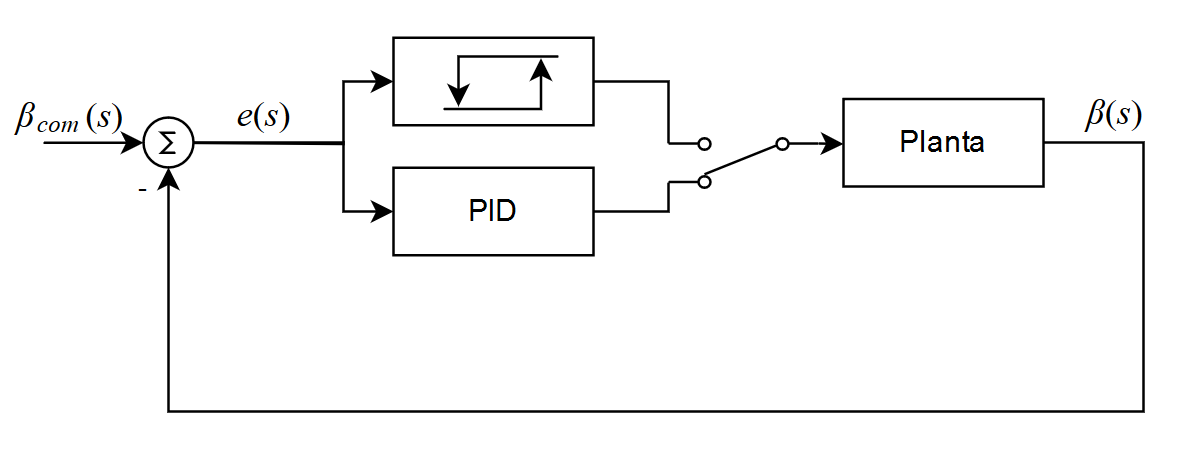
\includegraphics[scale=0.75]{img/pid_autotuning_relay_astrom_p239}
  \end{center}
  \fonte{Adaptado de \citeonline{Astrom1995}.} 
  \label{fig:pid_autotuning_relay_astrom_p239}
\end{figure}

O modelo matemático usado para descrever o comportamento de um relé, pode ser visto na equação da sequência que é obtida através da transformada de Fourier:

\begin{gather}
  N(a)=\frac{4d}{\pi a}\left(\sqrt{1-\left(\frac{\varepsilon}{a}\right)^{2}}-i\frac{\varepsilon}{a}\right) 
\end{gather}

Onde \textit{d} é a amplitude de oscilação do relé (normalmente até 10\% do sinal de referência), \textit{$\varepsilon$} é a histerese do relé e \textit{a} é a amplitude do sinal de referencia \cite{Levine1996}.

Com isso, podemos calcular os parâmetros intermediários para a sintonia do controlador da seguinte forma:

\begin{gather}
  K_u \approx \frac{4d}{\pi a} \\
  T_u = P_u
\end{gather}

Onde $P_u$ é o período de oscilação do sinal de interesse. Munido desses valores, podemos recorrer a tabela do método Ziegler-Nichols em resposta em frequência (Tabela \ref{tab:Ziegler-Nichols-freq}).

%%%%%%%%%%%%%%%%%%%%%%%%%%%%%%%%%%%
%\subsubsection{Método Baseado em Regras} %Astron 241


%%%%%%%%%%%%%%%%%%%%%%%%%%%%%%%%%%%%%%%%%%%%%%%%%%%%%%%%%%%%%%%%%%%%%%
\section{Sistemas Embarcados}

\begin{figure}[!ht]
  \caption{Estrutura Básica do Espaço de Usuário e de Kernel.}
  \begin{center}
      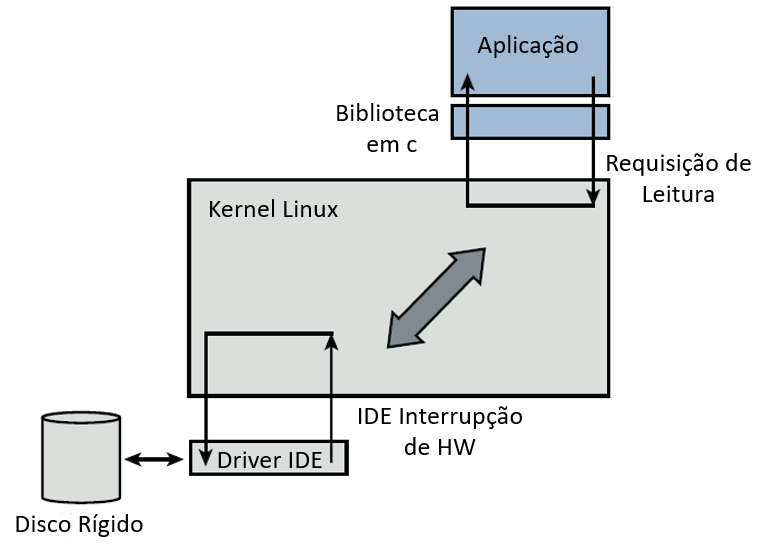
\includegraphics[scale=0.75]{img/kernel_user_space}
  \end{center}
  \fonte{Adaptado de Embarcados....} 
  \label{fig:kernel_user_space}
\end{figure}
  
\begin{figure}[!ht]
  \caption{Representação do Modelo de Controlador PID com distúrbios}
  \begin{center}
      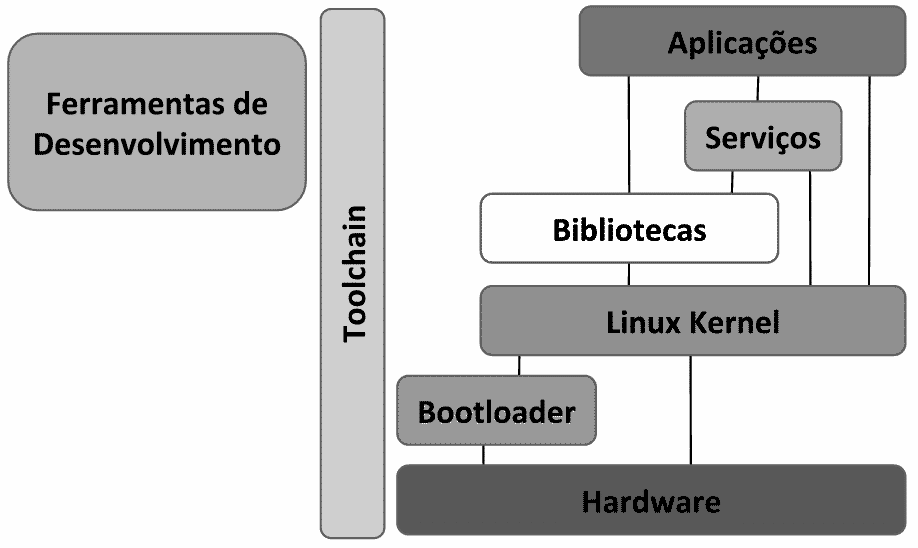
\includegraphics[scale=0.35]{img/sistema-linux-overview_embarcados}
  \end{center}
  \fonte{Adaptado de Embarcados....} 
  \label{fig:sistema-linux-overview_embarcados}
\end{figure}


%%%%%%%%%%%%%%%%%%%%%%%%%%%%%%%%%%%
\subsection{Comportamento Assíncrono}

%%%%%%%%%%%%%%%%%%%%%%%%%%%%%%%%%%%
\subsection{Escalonamento de Tarefas}

%%%%%%%%%%%%%%%%%%%%%%%%%%%%%%%%%%%
\subsection{Processamento Digital de Sinais}

\begin{figure}[!ht]
  \caption{Resposta ao degrau com diferentes períodos de amostragem.}
  \begin{center}
      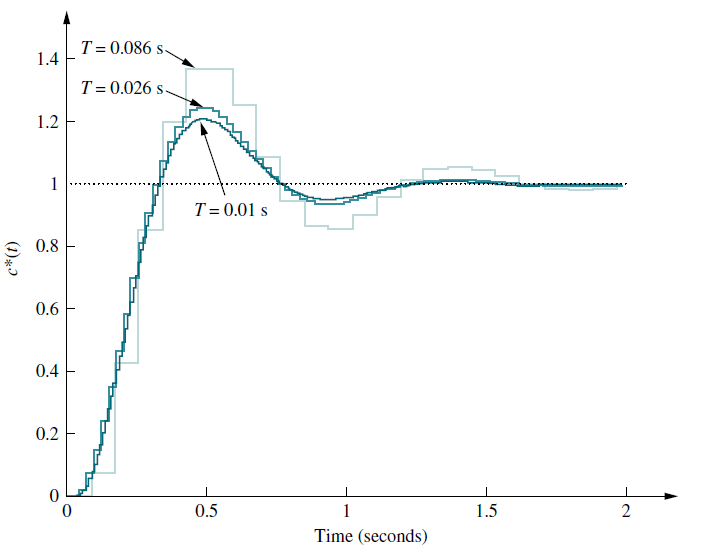
\includegraphics[scale=0.65]{img/nise_digitalinput_p761}
  \end{center}
  \fonte{Adaptado de \citeonline{Nise}.} 
  \label{fig:nise_digitalinput_p761}
\end{figure}

\subsubsection{Protocolos de MQTT e I2C}
%%%%%%%%%%%%%%%%%%%%%%%%%%%%%%%%%%%%%%%%%%%%%%%%%%%%%%%%%%%%%%%%%%%%%%
\section{Estado da Arte}

%%%%%%%%%%%%%%%%%%%%%%%%%%%%%%%%%%%
\subsection{Sistemas Inteligentes de Sintonia de Controladores}


\begin{figure}[!ht]
  \caption{Modelo de um Controlador com Auto-sintonia.}
  \begin{center}
      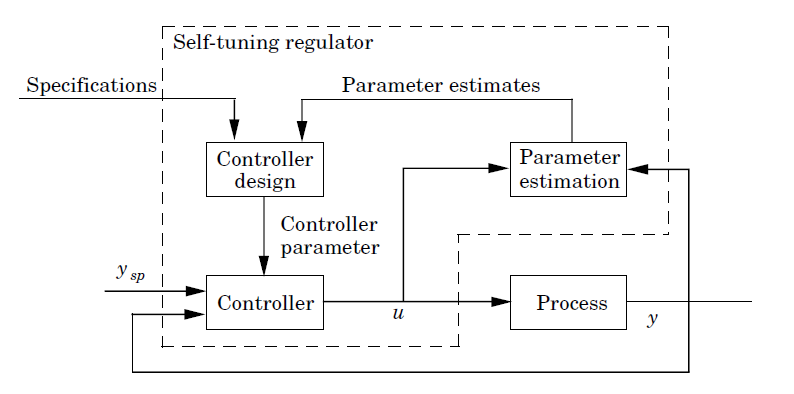
\includegraphics[scale=0.75]{img/pid_adaptative_astrom_p233}
  \end{center}
  \fonte{Adaptado de \citeonline{Astrom1995}.} 
  \label{fig:pid_adaptative_astrom_p233}
\end{figure}


%%%%%%%%%%%%%%%%%%%%%%%%%%%%%%%%%%%
\subsection{Controle Fuzzy} %Astrom p298


%%%%%%%%%%%%%%%%%%%%%%%%%%%%%%%%%%%
\subsection{Controle com Redes Neurais}  %control hand p1017

\begin{figure}[!ht]
  \caption{Modelo de um Simples Neurônio.}
  \begin{center}
      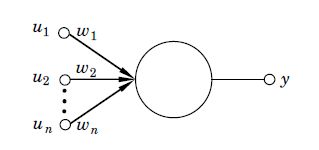
\includegraphics[scale=0.6]{img/neuron_astrom_p295}
  \end{center}
  \fonte{Adaptado de \citeonline{Astrom1995}.} 
  \label{fig:neuron_astrom_p295}
\end{figure}

\begin{figure}[!ht]
  \caption{Representação de uma Rede Neural.}
  \begin{center}
      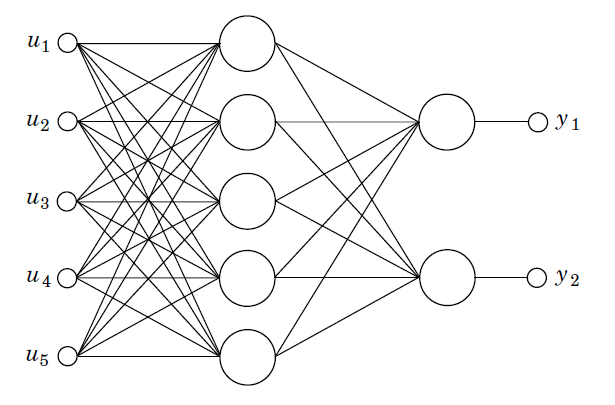
\includegraphics[scale=0.65]{img/feedforward_neural_astrom_p297}
  \end{center}
  \fonte{Adaptado de \citeonline{Astrom1995}.} 
  \label{fig:feedforward_neural_astrom_p297}
\end{figure}

\begin{figure}[!ht]
  \caption{Proposta de \citeonline{Chen2004} para um Controlador PID com Redes Neurais}
  \begin{center}
      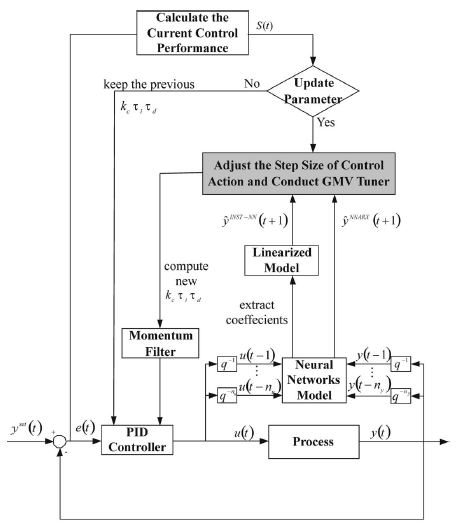
\includegraphics[scale=1]{img/pid_neural_Applying_p18}
  \end{center}
  \fonte{Adaptado de \citeonline{Chen2004}.} 
  \label{fig:pid_neural_Applying_p18}
\end{figure}

%%%%%%%%%%%%%%%%%%%%%%%%%%%%%%%%%%%%%%%%%%%%%%%%%%%%%%%%%%%

\cite{Verma2018}
\cite{Li2010}
\cite{Nise}
\cite{Chen2004}
\cite{Liguo2008}
\cite{Amaral}
\cite{Araari2014}
\cite{Rolle2009}
\cite{Li}
\cite{Ogata}
\cite{Snider}
\cite{Gohiya2012}
\cite{Hu2001}
\cite{Johnson}
\cite{Editor}
\cite{Li2013}
\cite{Das2017}
\cite{Dorf}
\cite{Levine1996}
\cite{Thomas}
\cite{Guo2010}
\cite{Liu2011}
\cite{Astrom1995}
\cite{Behera2017}
\cite{Brown2002}